%!TEX TS-program = xelatex
%!TEX encoding = UTF-8 Unicode

\documentclass[11pt,tikz,border=1]{standalone}
\usetikzlibrary{positioning}

\begin{document}
  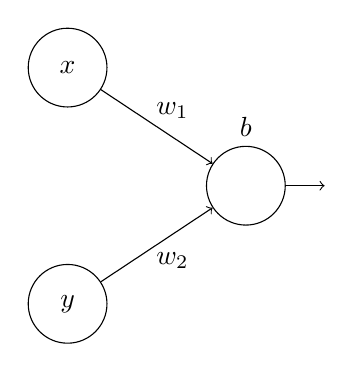
\begin{tikzpicture}[
    neuron/.style={circle,draw,inner sep=0pt,minimum size=10mm}
    ]
    
    \node(n) [neuron] {};
    \node(x) [neuron,left=1.25 of n,yshift=1.5cm] {$x$};
    \node(y) [neuron,left=1.25 of n,yshift=-1.5cm] {$y$};
    
    \draw[->] (x) -- node [yshift=2mm,xshift=2mm] {$w_1$} (n);
    \draw[->] (y) -- node [yshift=-2mm,xshift=2mm] {$w_2$} (n);
  
    \node [above] at (n.north) {$b$};
    \draw[->] (n) -- ++(1cm, 0);
    
  \end{tikzpicture} 
\end{document}
